\documentclass[12pt]{article}
\usepackage[english]{babel}
\usepackage{sbc-template}
\usepackage{graphicx,url}
\usepackage[utf8]{inputenc}
\usepackage[ruled,vlined]{algorithm2e}
\DontPrintSemicolon
\SetAlgoLined
\SetKwFunction{BMILS}{BM-ILS}
\SetKwFunction{Preprocessing}{\(PreProcessing\)}
\SetKwFunction{ComputeBounds}{\(ComputeBounds\)}
\SetKwFunction{ConstructInitialSolution}{\(ConstructInitialSolution\)}
\SetKwFunction{BMLS}{\(BM-LS\)}
\SetKwFunction{DestroyShrinkRepair}{\(DestroyShrinkRepair\)}
\SetKwProg{Fn}{function}{:}{}
     
\sloppy

\title{A GRASP based approach for the Bin Packing Problem with General Precedence Constraints}

\author{Carlos E. Aguiar\inst{1}, Pedro Saccomani\inst{1}, Rangel Á. Barroso\inst{1} }


\address{Departamento de Ciência da Computação \\ Universidade Federal de Minas Gerais  (UFMG) -- Belo Horizonte, MG -- Brazil
  \email{Caduaguiar.roma@gmail.com, psaccomani15@gmail.com,
  rangel-avila@ufmg.br}
}

\begin{document} 

\maketitle

% \begin{abstract}
%   This meta-paper describes the style to be used in articles and short papers
%   for SBC conferences. For papers in English, you should add just an abstract
%   while for the papers in Portuguese, we also ask for an abstract in
%   Portuguese (``resumo''). In both cases, abstracts should not have more than
%   10 lines and must be in the first page of the paper.
% \end{abstract}
     
% \begin{resumo} 
%   Este meta-artigo descreve o estilo a ser usado na confecção de artigos e
%   resumos de artigos para publicação nos anais das conferências organizadas
%   pela SBC. É solicitada a escrita de resumo e abstract apenas para os artigos
%   escritos em português. Artigos em inglês deverão apresentar apenas abstract.
%   Nos dois casos, o autor deve tomar cuidado para que o resumo (e o abstract)
%   não ultrapassem 10 linhas cada, sendo que ambos devem estar na primeira
%   página do artigo.
% \end{resumo}


\section{Introduction}
% Contextualization
In modern software development environments, organizations face increasingly complex challenges in managing the delivery of software features across multiple development cycles and deployment windows.

Software teams must regularly decide how to group and schedule features for delivery, while respecting complex dependencies between components, modules, and functionalities. This real-world scenario mirrors a classic combinatorial optimization challenge, where limited resources (delivery windows, development capacity, testing environments) must be allocated efficiently while maintaining the correct execution order of interdependent tasks.

The complexity intensifies when considering that resources often have sizes, priorities, and precedence relationships that cannot be violated during the delivery process.

% Problem Definition
The Bin Packing Problem with General Precedence Constraints (BPP-GP) can be formally defined as follows: given a set of items $N = \{1,2,...,n\}$ with associated weights $w_j$, a set of identical bins with capacity $C$, subject to a set of precedence constraints between item pairs that define their partial order relationships, the objective is to pack all items into the minimum number of bins, ensuring that no bin exceeds its capacity and that all precedence relationships are respected within a bin and across bins.

This optimization problem extends the classical bin packing problem by incorporating ordering dependencies that are fundamental in software development contexts.

% Problem Characterization - Complexity Class
The Bin Packing Problem with General Precedence Constraints belongs to the class of NP-Hard optimization problems. This classification arises from the fact that even the basic bin packing problem without precedence constraints is NP-Hard, and the addition of these constraints only allows for the description of more expressive problems.

The decision version of this problem, which asks whether there exists a feasible packing using at most $k$ bins while respecting all constraints, is NP-Complete, making it unlikely that polynomial-time exact algorithms exist to solve large instances of this problem.

% Problem Characterization - Similar Problems
Several related problems share structural similarities with BPP-GP, including the classical Bin Packing Problem (without precedence constraints), the Job Shop Scheduling Problem with precedence constraints, the Resource-Constrained Project Scheduling Problem (RCPSP), and the Knapsack Problem with Precedence Constraints.

Furthermore, variants such as the Bin Packing Problem with Conflicts, where certain items cannot be placed in the same bin, and the Multidimensional Bin Packing Problem provide insights into techniques for handling constraints.

The Strip Packing Problem with precedence constraints also offers relevant algorithmic approaches, particularly in the context of scheduling and resource allocation.

%  Problem Characterization - Additional Relevant Information
BPP-GP presents several unique features that distinguish it from standard combinatorial optimization problems. Precedence constraints create a partial ordering that can result in complex dependency graphs, potentially including parallel branches and multiple hierarchy levels. In software delivery contexts, these constraints may represent technical dependencies, business priorities, relationships between user stories, or testing requirements. The problem allows for intra-bin precedence (dependencies within the same delivery window) and inter-bin precedence (dependencies spanning multiple delivery cycles), significantly complicating the solution space and requiring sophisticated constraint propagation mechanisms.

% Motivation
This problem deserves investigation due to its direct applicability to critical challenges in modern software engineering and project management. As software systems become increasingly complex and development teams adopt agile methodologies with frequent delivery cycles, the efficient allocation of resources to delivery windows while respecting dependencies becomes fundamental to project success. Inadequate scheduling of resources can lead to development bottlenecks, release delays, inefficient resource utilization, and increased technical debt.

Furthermore, the investigation of a meta-heuristic based approach for such problem can advance the broader field of combinatorial optimization with constraints and provide insights applicable to other domains, such as supply chain management, manufacturing scheduling, and resource allocation problems.

% Objectives
This research builds upon the baseline methodology proposed by \cite{kramer:17} for the Bin Packing Problem with General Precedence Constraints (BPP-GP). The original approach provides a structured framework for addressing precedence-aware packing through iterative local search techniques. In this work, we take this baseline as a starting point and extend it by implementing a GRASP-based metaheuristic, aiming to enhance the efficiency of precedence propagation and packing strategies. The objective remains to minimize the number of bins while ensuring feasibility with respect to both intra-bin and inter-bin dependencies, leveraging the strengths of the baseline while exploring improvements through the GRASP methodology.

% Justification
The justification for this work lies both in its practical relevance and in the theoretical contribution it may offer. In practice, the optimization of software resource delivery under precedence constraints addresses a real need faced by development teams, where the complexity of manual scheduling often leads to inefficiencies and delays. From a theoretical perspective, the formulation and analysis of heuristics for BPP-GP expand the body of knowledge in combinatorial optimization under complex constraints, providing new perspectives that may be applied in domains beyond software engineering, such as logistics, manufacturing, and project management. Thus, the research is justified by its ability to generate direct impact on critical engineering processes while simultaneously strengthening the academic understanding of NP-Hard problems with additional constraints.

% Roadmap
The development of this work will follow a structured roadmap in progressive steps, as follows:
\begin{itemize}
  \item \textbf{Literature review:} Investigation of the BPP-GP problem and related combinatorial optimization problems, with emphasis on metaheuristic strategies previously applied in similar contexts, including the baseline proposed by \cite{kramer:17};
  \item \textbf{Problem definition:} Formal and computational description of the BPP-GP, highlighting its constraints, objectives, and relevance to resource allocation and scheduling problems;
  \item \textbf{Development of the metaheuristic algorithm:} Design and implementation of a new metaheuristic approach to replace or extend the baseline method proposed in \cite{kramer:17}, aiming to improve solution quality and robustness. Particular attention will be given to mechanisms that effectively manage precedence constraints;
  \item \textbf{Definition of the experimental methodology:} Establishment of the experimental protocol, including test instance selection or generation, parameter tuning strategies, performance metrics, and reference algorithms for comparison;
  \item \textbf{Execution of computational experiments:} Implementation, execution, and evaluation of the proposed metaheuristic on benchmark instances. The results will be analyzed in terms of computational efficiency, convergence behavior, and quality of the obtained solutions, with comparisons to baseline and state-of-the-art methods;
  \item \textbf{Conclusions and future research directions:} Summary of the main findings and assessment of the proposed metaheuristic’s effectiveness in solving the BPP-GP. Limitations will be discussed, and perspectives for future work will be outlined, such as algorithmic refinements, hybridizations with other techniques, or applications to extended problem variants.
\end{itemize}

\newpage
\section{Related work}

The Bin Packing Problem with Precedence Constraints (BPP-P) can be can be seen as an extension to the well known Bin Packing Problem in order to incorporate precedence constraints. A BPP-P instance is described by a set of items \(N = {1, 2, \dots, n}\), with non-negative weights and a set of bins \(M = {1, 2, \dots, m}\), each with capacity \(C\). In addition to that, in the set of items, there is also a \textbf{precedence} relation. The goal is to pack all items in the bins respecting the capacity and the precedence: items with less precedence must be packed into lower numbered bins.

 A solution to this problem was introduced in the work of \cite{dell2012bin}. They consider different, independent approaches: 
 A branch-and-bound procedure, a greedy constructive heuristic (first fit), together with a local search procedure, and also a 
 \textit{Variable Neighborhood Search}.

 Focusing on the classic problem in the same year, the work by \cite{layeb:12} addresses the one-dimensional Bin Packing Problem (1-BPP), 
 the simplest version of the problem. The authors propose a new approach based on the GRASP (Greedy Randomized Adaptive Search Procedure) 
 meta-heuristic. The methodology is implemented in two phases: the first is a construction phase that uses a new randomized greedy heuristic, 
 notable for being a hybrid between the First Fit (FF) and Best Fit (BF) heuristics; the second phase consists of a local search based on 
 the Tabu Search (TS) algorithm, used to refine and improve the solution found in the first phase. The experimental results, conducted on 
 benchmark instances (easy, medium, and hard), demonstrate that the proposed GRASP approach significantly outperforms the simple greedy 
 heuristic and achieving results very close to the best-known solutions.

The work by \cite{pereira:16} proposes a heuristic based on dynamic 
programming and an exact branch-and-bound method, incorporating several new lower bounds and dominance
rules to improve performance. The computational results show the notable effectiveness of the 
proposed methods, which were able to find the optimal solution for all previously unsolved ("open") 
instances from the classic benchmark set, significantly outperforming prior approaches in terms of 
solution quality and speed. The study concludes that the developed procedures represent the new 
state-of-the-art, and it identifies that instances with large item weights and a low number of 
precedence relations (low order strength) are the most challenging for the algorithm.

Later, the work of \cite{kramer:17} proposes an extension of this problem, the Bin Packing Problem with general precedence constraints, which is the topic of interest of our research project. This problem further generalizes the BPP-P by introducing weighted precedences: Each precedence relation between items \(a\) and \(b\) is described by a tuple \((a, b)\) with an associated integer \(t\), the goal is to have \(i_a - i_b \geq t\), where \(i_a\) and \(i_b\) are the bins where \(a, b\) are inserted. This work also introduces a simple algorithm, based on the \textit{Iterated Local Search} procedure. Using a set of constructive heuristics to build an initial solution that are then refined. The computational results show that the proposed method, is robust and provides high-quality solutions within a 
reasonable time, comparing well with state-of-the-art methods tailored for particular problem cases. The authors conclude that their simple and flexible approach is effective, although the introduction
of heterogeneous precedences presents new challenges for both exact and heuristic methods, 
leaving many instances unsolved to proven optimality and suggesting avenues for future research.

Expanding on the application of heuristics for similar optimization problems, \cite{lalaoui:18} address 
the Simple Assembly Line Balancing Problem of type I (SALBP-I) by proposing an adaptive metaheuristic. 
Their approach employs a generalized simulated annealing algorithm whose parameters are dynamically 
adjusted by a fuzzy inference system, aiming to quickly find effective solutions for rebalancing 
production lines in response to factors like demand fluctuation. The paper's conclusion is based on 
the performance analysis of their fuzzy simulated annealing method on a well-known benchmark dataset 
for SALBP-I, demonstrating its applicability in minimizing the number of workstations for a given 
cycle time.

The existing literature presents robust methods for the Bin Packing Problem with Generalized Precedence Constraints (BPP-GP) and its variants.
 Notably, \cite{kramer:17} proposed an effective baseline method for the BPP-GP based on Iterated Local Search (ILS). Concurrently, other 
 metaheuristics have demonstrated great success on similar problems, such as GRASP, which was effectively applied by \cite{layeb:12} to the 
 classic 1-BPP. While the ILS approach from \cite{kramer:17} serves as an established benchmark, the success of GRASP in combinatorial 
 optimization motivates its application to the BPP-GP.

This project aims to extend the baseline method proposed in \cite{kramer:17} by developing and integrating an adapted GRASP metaheuristic, 
which will replace the original ILS procedure to explore a new solution pathway for this complex problem.

\newpage
\section{Methodology}

In this work, we will implement a GRASP approach which uses ideas from the work of \cite{kramer:17}. We will use this same study as our control method. The authors of this study propose an algorithm based on Iterated local search, as presented below:

\begin{algorithm}[H]
  \footnotesize
\Fn{\BMILS{$Instance$}}{
    $ImprovedInstance \leftarrow$ \Preprocessing{$Instance$}\;
    $LB \leftarrow$ \ComputeBounds{$ImprovedInstance$}\;
    \tcc*[h]{Construct first solution}\;
    $x_{incumbent} \leftarrow$ \ConstructInitialSolution{$ImprovedInstance$}\;
    $x_{best} \leftarrow x_{incumbent}$\;
    \Repeat{$z(x_{best}) = LB$ \textbf{or} Timeout()}{
      \tcc*[h]{Intensification using batch of moves}\;
        $x_{incumbent} \leftarrow$ \BMLS{$x_{incumbent}$} 
        \If{$z(x_{incumbent}) < z(x_{best})$}{
            $x_{best} \leftarrow x_{incumbent}$\;
        }
        $\rho \leftarrow random(1, K\_MAX(ImprovedInstance))$\;
        $x_{incumbent} \leftarrow$ \DestroyShrinkRepair{$x_{incumbent}, \rho$} \tcp*[r]{Diversification}
    }
    \Return{$x_{best}$}\;
}
\caption{Control Metaheuristic}
\end{algorithm}

This algorithm is comprised of three main phases:
\begin{enumerate}
  \item Pre-Processing and lower-bound computation: This phase contributes to a speed-up in the convergence of the algorithm. They adapt the procedures presented in \cite{dell2012bin}.
  \item Initial Solution Computation: The procedure employ two independent \textbf{greedy constructive} heuristics and a linear integer programming approach. At the end, the best solution is selected.
  \item Local Search: The goal of this phase is to refine the initial solution either until we reach a fixed timeout or reach the lower bound. 
\end{enumerate}

In our work, we plan to construct a GRASP based approach derived from this prior work. Each iteration of the GRASP metaheuristic contains two main steps:
\begin{itemize}
  \item Construction of initial solutions: In this step, a feasible solution is built using a \textbf{randomized adaptative greedy} algorithm.
  \item Local-Search step: This initial solution is refined until a local optima is reached. 
 \end{itemize}

 This randomized greedy algorithm is controlled by a parameter \(\alpha\) which defines the compromise between search exploitation and exploration. In our work, this \(\alpha\) will be adaptative, that is, its value will be tuned through the procedure.

 In the constructive step, we plan to adapt the two greedy constructive heuristics employed by \cite{kramer:17} to be randomized in order to be incorporated into a GRASP step. We will also explore other possible heuristics that could bring benefits to our approach. In the local search step, we plan to use the local search (BM-LS) algorithm also proposed by \cite{kramer:17}.

 We hope that our work could produce at least comparable solutions to \cite{kramer:17} given the same execution times, and in some cases even better solutions to some benchmarks, due to the explorative/adaptative factor in GRASP.
 
 \subsection{Evaluation}

 For this phase, we will utilize already propose benchmarks sets for this problem. The work of \cite{kramer:17} also expands a standard benchmark set proposed by \cite{otto:13}. We plan to ask the authors of such work in order to use this extended set.

 During our work, we will employ some intermediate evaluation steps, to decide how we should handle the use of the constructive heuristics, trying to answer the question: ``Should we be inspired by \cite{kramer:17} and also run both, selecting the better result or should we also employ some randomness in this selection?''.

 After completing this implementation phase, we will compare our approach with established techniques in the literature, such as the Iterated Local Search method proposed by \cite{kramer:17} and other state-of-the-art metaheuristics for the BPP-GP problem. The comparison will focus on both solution quality and computational efficiency.

To ensure a rigorous evaluation, we will adopt the following methodology:
\begin{itemize}
\item \textbf{Performance metrics:} We will consider multiple measures of solution quality, including the number of bins used, average gap to 
the known lower bounds, and the distribution of solution values across multiple runs. Computational efficiency will be assessed through CPU 
time, number of iterations, and convergence behavior.
\item \textbf{Statistical analysis:} To account for the stochastic nature of GRASP, each experiment will be repeated multiple times 
(e.g., 10 independent runs), and results will be statistically analyzed. Metrics such as mean, standard deviation, and confidence intervals 
will be reported.
\item \textbf{Benchmark instances:} Experiments will be conducted on standard benchmark sets, including the extended set from 
\cite{kramer:17} and the original set from \cite{otto:13}. Instances will cover a wide range of sizes and complexity levels to assess the 
scalability and robustness of the algorithm.
\item \textbf{Parameter tuning:} Sensitivity analysis will be conducted for key algorithmic parameters, particularly the adaptive \(\alpha\) 
controlling the randomized greedy construction, to identify configurations that maximize performance.
\item \textbf{Ablation studies:} To understand the contribution of each component of the GRASP approach (e.g., randomized constructive 
heuristics, BM-LS local search, adaptive \(\alpha\)), we will perform ablation experiments by selectively removing or 
modifying components and observing their impact on solution quality and convergence.
\end{itemize}

This evaluation framework aims to provide a thorough and fair comparison between our proposed GRASP metaheuristic and existing methods, 
highlighting potential improvements in solution quality, robustness, and computational efficiency. By combining detailed performance metrics 
with statistical analysis and controlled experiments, we aim to draw rigorous conclusions about the effectiveness of the proposed approach for 
the BPP-GP problem.

 % Depois seria bom dar uma revisada no que coloquei, mas achei justo (talvez algumas coisas dê mt trabalho, aí cortamos posteriormente)
 % Ver também se está razoável com o que ele pede no roteiro

\newpage
\section{Schedule}

To ensure a structured and timely execution of this research, the project has been divided into distinct stages, each with defined tasks, 
deadlines, and assigned responsibilities. Table~\ref{tab:schedule} presents the detailed schedule, including the duration of each stage 
and the collaborators responsible for its completion. This structured timeline provides a clear roadmap for implementing the baseline, 
developing the proposed GRASP metaheuristic, conducting experiments, analyzing results, and preparing the final deliverables.

% Cronograma foi feito para encaixar nos 28-30 dias que temos. As tasks coloquei aleatoriamente, só para preencher a tabela

\begin{table}[ht]
\caption{Project Schedule and Responsibilities}
\label{tab:schedule}
\begin{tabular}{clccc}
\hline
\textbf{Stage} & \textbf{Task} & \textbf{Deadline} & \textbf{Duration} & \textbf{Responsible} \\ \hline
1 & Review and Planning & 27--29 Oct & 3 days & Rangel \\
2 & Baseline Implementation & 30 Oct--2 Nov & 4 days & Carlos \\
3 & New Implementation & 3--7 Nov & 5 days & Carlos \\
4 & Integration and Debugging & 8--10 Nov & 3 days & Carlos, Pedro \\
5 & Execution of Experiments & 11--14 Nov & 4 days & Pedro \\
6 & Results Analysis & 15--17 Nov & 3 days & Pedro, Rangel \\
7 & Article Writing & 18--22 Nov & 5 days & Rangel \\
8 & Presentation and Final Review & 23--25 Nov & 3 days & All \\ \hline
\multicolumn{2}{l}{\textbf{Total}} & & \textbf{30 days} & \\ \hline
\end{tabular}
\end{table}




%% Restante do código está comentado para renderizar somente até a parte feita %%

% \section{First Page} \label{sec:firstpage}

% The first page must display the paper title, the name and address of the
% authors, the abstract in English and ``resumo'' in Portuguese (``resumos'' are
% required only for papers written in Portuguese). The title must be centered
% over the whole page, in 16 point boldface font and with 12 points of space
% before itself. Author names must be centered in 12 point font, bold, all of
% them disposed in the same line, separated by commas and with 12 points of
% space after the title. Addresses must be centered in 12 point font, also with
% 12 points of space after the authors' names. E-mail addresses should be
% written using font Courier New, 10 point nominal size, with 6 points of space
% before and 6 points of space after.

% The abstract and ``resumo'' (if is the case) must be in 12 point Times font,
% indented 0.8cm on both sides. The word \textbf{Abstract} and \textbf{Resumo},
% should be written in boldface and must precede the text.

% \section{CD-ROMs and Printed Proceedings}

% In some conferences, the papers are published on CD-ROM while only the
% abstract is published in the printed Proceedings. In this case, authors are
% invited to prepare two final versions of the paper. One, complete, to be
% published on the CD and the other, containing only the first page, with
% abstract and ``resumo'' (for papers in Portuguese).

% \section{Sections and Paragraphs}

% Section titles must be in boldface, 13pt, flush left. There should be an extra
% 12 pt of space before each title. Section numbering is optional. The first
% paragraph of each section should not be indented, while the first lines of
% subsequent paragraphs should be indented by 1.27 cm.

% \subsection{Subsections}

% The subsection titles must be in boldface, 12pt, flush left.

% \section{Figures and Captions}\label{sec:figs}


% Figure and table captions should be centered if less than one line
% (Figure~\ref{fig:exampleFig1}), otherwise justified and indented by 0.8cm on
% both margins, as shown in Figure~\ref{fig:exampleFig2}. The caption font must
% be Helvetica, 10 point, boldface, with 6 points of space before and after each
% caption.

% \begin{figure}[ht]
% \centering
% 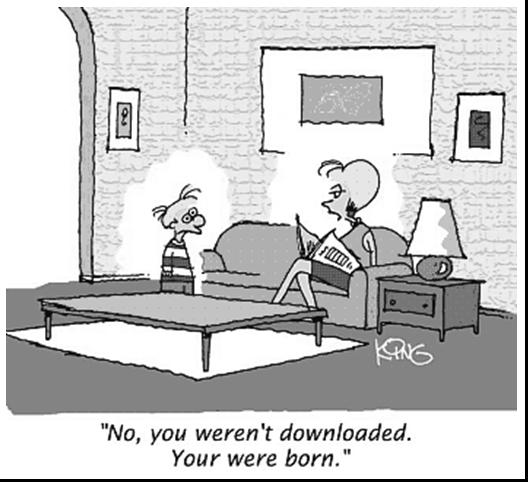
\includegraphics[width=.5\textwidth]{fig1.jpg}
% \caption{A typical figure}
% \label{fig:exampleFig1}
% \end{figure}

% \begin{figure}[ht]
% \centering
% 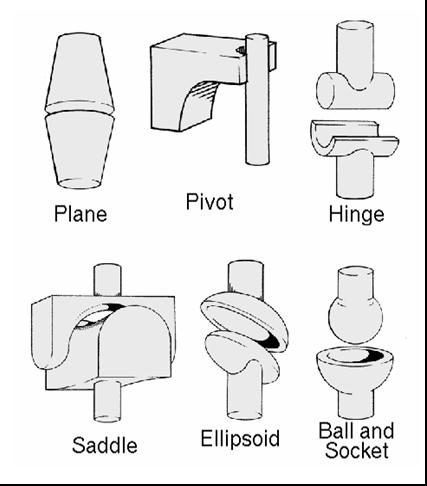
\includegraphics[width=.3\textwidth]{fig2.jpg}
% \caption{This figure is an example of a figure caption taking more than one
%   line and justified considering margins mentioned in Section~\ref{sec:figs}.}
% \label{fig:exampleFig2}
% \end{figure}

% In tables, try to avoid the use of colored or shaded backgrounds, and avoid
% thick, doubled, or unnecessary framing lines. When reporting empirical data,
% do not use more decimal digits than warranted by their precision and
% reproducibility. Table caption must be placed before the table (see Table 1)
% and the font used must also be Helvetica, 10 point, boldface, with 6 points of
% space before and after each caption.
% \section{Images}

% All images and illustrations should be in black-and-white, or gray tones,
% excepting for the papers that will be electronically available (on CD-ROMs,
% internet, etc.). The image resolution on paper should be about 600 dpi for
% black-and-white images, and 150-300 dpi for grayscale images.  Do not include
% images with excessive resolution, as they may take hours to print, without any
% visible difference in the result. 

% \section{References}

% Bibliographic references must be unambiguous and uniform.  We recommend giving
% the author names references in brackets, e.g. \cite{knuth:84},
% \cite{boulic:91}, and \cite{smith:99}.

% The references must be listed using 12 point font size, with 6 points of space
% before each reference. The first line of each reference should not be
% indented, while the subsequent should be indented by 0.5 cm.

\bibliographystyle{sbc}
\bibliography{sbc-template}

\end{document}
